\documentclass[12pt]{jarticle}
\usepackage[a4paper,text={155mm,230mm},centering]{geometry}
\usepackage{amssymb,amsmath,amsthm}
%\usepackage[dvips]{graphicx}
\usepackage{fancyhdr}
\pagestyle{fancy}
\lhead{ワイヤレス給電システムの最適化のための能率的な動作周波数スイープ}
\chead{}
\rhead{\thepage}
\lfoot{}
\cfoot{}
\rfoot{森田光流}
\usepackage{fancybox}
\usepackage{listings,jlisting}
\usepackage{color}
\usepackage{ascmac, here, txfonts, txfonts}
\usepackage[dvipdfmx]{graphicx}


\begin{document}
	
%%%%%%%%%%%%%%%%%%%%%%%%%%%%%%%%%表紙
\thispagestyle{empty}

\vspace*{20mm}
\begin{center}
	{\Large 令和元年度 環境ロボティクス学科 卒業論文}
\end{center}
\vspace{10mm}
\begin{center}
	{\Huge ワイヤレス給電システムの最適化のための能率的な動作周波数スイープ}
\end{center}
\vspace{90mm}
\begin{center}
	{\Large 令和2年 (2020) 2月14日}
\end{center}
\begin{center}
	{\Large 森田 光流}
\end{center}
\begin{center}
	{\Large 指導教員:穂高一条教授}
\end{center}

\clearpage
%%%%%%%%%%%%%%%%%%%%%%%%目次

\tableofcontents

\clearpage
%%%%%%%%%%%%%%%%%%%%%%%本文

\section{緒言}
\subsection{背景}
\subsubsection{ワイヤレス給電の概要}
ワイヤレス給電とは,コネクタや金属接点の接触を用いず無線で電力を供給,伝搬することが可能な給電方法である.非接触充電,非接触電力送電,無線給電などとも呼ばれている.従来の電気製品の給電方法の金属接点やコネクタを使用したものは,水がかかると水による感電やショートを起こす,配線による転倒などの安全面に関して問題点がある.しかしワイヤレス給電は金属接点が非接触なので前述に述べた安全面の問題点の解決するだけではなく,人が立ち入れない危険な場所にある機器や装置の遠隔操作ができるなどという利点が期待されており,現在盛んに研究されている.
\subsubsection{ワイヤレス給電の特徴}
ワイヤレス給電が無線で電力を供給するためには,送電側と受電側の2つのコイルを用いるため物理的な金属接点やコネクタが存在せず,また非金属のものであれば,コイル間に存在していても送電側と受電側の電力に影響を及ぼさない.また,送電コイルを表面に露出させる必要がないため,水による感電やショートする心配がないので,水場での使用が可能である.なお,ワイヤレス給電の給電方式には送電側と受電側との間発生する誘導磁束を利用した電磁誘導方式や,キャパシタを送電電極と受電電極として電力を送電する電解結合方式などがある\cite{rohm2}\cite{ito}が,本研究ではその中の電磁共鳴方式で行う.
\subsubsection{ワイヤレス給電の将来性}
現在,ワイヤレス給電の特徴を生かして様々な場所に導入しようと 研究が行われている.前述に述べた通り金属接点が非接触なので,ワイヤレス給電化することにより物理的な金属接点が少なくなるので電源コードは最小限で済み余分な空間を作ることにより直接配線などの問題解決並びに自動化・効率化に大きく貢献している\cite{syourai}\cite{matuda}.
\\ また,地球温暖化の影響によりCO{\tiny 2}の削減のため電気自動車開発並びに普及が望まれている.現在,電気自動車に使用されている接触式充電方式は雨天時にプラグを扱うと感電する可能性がある.それをワイヤレス給電に置き換えると自宅の駐車場に駐車するだけで充電が可能になり電の可能性が払拭される,充電の際に運転者が降車する必要がなくなり運転者の負担が大きく軽減されることが期待される.\cite{hakugin}
\clearpage
\subsection{研究目的}
ワイヤレス給電の電力供給の効率の改善には,
\\1.最適な周波数調整
\\2.結合操作
\\3.マルチループコイルとLC回路を用いた適応マッチング
\\などがある\cite{morita}.本研究においては1.に注目し,そのために最適動作周波数の探索をすることとした.1.を最適動作周波数を探索するには,受電電力と送電電力を使った電力効率を求める必要がある.しかし,電力効率が高いだけでは最適動作周波数が適切であるとはいえない.受電側と送電側の元々の電力が小さい場合も電力効率が高いということが考えられる.それではワイヤレス給電が最適に動作しているとは考えられない.したがって,最適動作周波数は高効率かつ大電力が出力される周波数と定義される.
\\ また最適動作周波数を探索するためには多くの周波数データ測定しなければいけないので測定時間をなるべく短くしたい.しかし,ワイヤレス給電に周波数を送った後,安定な電力が出力されるまで時間がかかる.したがって%本研究は能率的な周波数スイープ作成並びに,
ワイヤレス給電システムの最適動作周波数を能率的な周波数スイープによる測定,考察を目的にした.
\clearpage
\section{本論文の構成}

\clearpage
\section{原理}
\subsection{ワイヤレス給電の原理}
\begin{figure}[h]
	\centering
	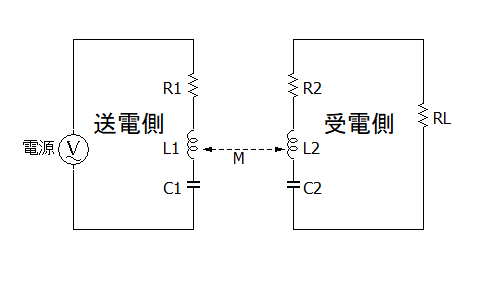
\includegraphics[]{wpt_2020128.png}
	\caption{ワイヤレス給電回路図}
	\label{fig:wpt_kairo}
\end{figure}
本研究で扱うワイヤレス給電の回路は図\ref{fig:wpt_kairo}で示される.図\ref{fig:wpt_kairo}に示すように,ワイヤレス給電は送電側の
\section{実験内容}

\section{実験結果}

\section{考察}

\section{結論}

\section{今後の展望}

\clearpage
\section{謝辞}
 本研究の進行や本論文等の執筆にあたり,ご指導いただいた穂高一条教授に感謝の意を示すとともに深く御礼申し上げます.
また本研究を進めるにあたり多大なご指導・助言してくださった自動制御研究室の先輩方並びに,共に研究した同期のメンバー
にも感謝の意を示すとともに深く御礼申し上げます.最後になりましたが,お世話になりました宮崎大学工学部環境ロボティクス
学科の先生方,並びに大学関係各位の皆様に心より感謝し,ここに御礼申し上げます.

\begin{thebibliography}{50}
	\bibitem{matuda}松田一志:”ワイヤレス給電システムのための電力測定回路の開発”,宮崎大学学士論文,平成30年度
	\bibitem{nakamura}中村裕馬:”ワイヤレス給電のための送電側100kHzプッシュプル回路”,宮崎大学学士論文,平成30年度
	\bibitem{rohm1}ローム株式会社:”ワイヤレス給電とは”ーエレクトロニクス豆知識, https://www.rohm.co.jp/electronics-basics/wireless-charging/wireless-charging\_what1,最終アクセス:2020/1/20
	\bibitem{rohm2}ローム株式会社:"ワイヤレス給電(無線給電)方式"ーエレクトロニクス豆知識, https://www.rohm.co.jp/electronics-basics/wireless-charging/wireless-charging\_what2
	\bibitem{tkinter}keicode.com-技術入門シリーズ:"TkinterによるGUIプログラミング"ーPython入門,https://python.keicode.com/advanced/tkinter.php, 最終アクセス:2020/1/21
	\bibitem{goizuka}五位塚潤:"低周波数域駆動によるワイヤレス給電回路", 宮崎大学学士論文, 平成29年度
	\bibitem{hakugin}白銀聡一郎:"ワイヤレス給電のための短形波電源装置の設計と開発",宮崎大学学士論文,平成29年度
	\bibitem{morita}盛田穣文:"ワイヤレス給電システムの効率と電力の最適化について", 宮崎大学修士論文, 平成29年度
	\bibitem{ito}伊東雅浩:"短径波入力による高効率ワイヤレス給電の制御について", 宮崎大学修士論文, 平成30年度
	\bibitem{syourai}B\&PLUS:"ワイヤレス給電の現状と未来",https://www.b-plus-kk.jp/about/mechanism.html 最終アクセス:2020/1/23
\end{thebibliography}
\clearpage
\section{付録}
\subsection{プログラムについて}
前章に示された通り先行研究では周波数を変更する方法で,わざわざArduinoのプログラムの一部を変更して再コンパイルさせ出力結果をシリアルモニターに表示させる方法であった.その面倒を省くためpythonを利用して周波数をarduinoに送り,arduinoの出力結果をデータに保存させるGUIを作成した.以下のプログラムはGUIで周波数をarduinoへシリアル通信で送信してarduinoに出力されたデータをシリアル通信でpython側に送る流れをするための,それぞれGUIのpythonプログラムと送電側のマイコンのarduinoプログラム,受電側のarduinoプログラムである.なお,pythonのプログラムにおいてGUIを作成にtkinterを使用した.tkinterの使用方法並びにpythonの使い方については参考文献:\cite{tkinter}を参考にした.
\lstset{
	%プログラム言語(複数の言語に対応,C,C++も可)
	backgroundcolor={\color[gray]{.90}},
	breakindent = 10pt,
	basicstyle = \ttfamily\scriptsize,
	commentstyle = {\itshape \color[cmyk]{1,0.4,1,0}},
	classoffset = 1,
	keywordstyle = {\bfseries \color[cmyk]{0,1,0,0}},
	stringstyle = {\ttfamily \color[rgb]{0,0,1}},
	frame = TBrl,
	framesep = 5pt,
	numbers = left,
	stepnumber = 1,
	numberstyle = \tiny\sffamily,
	tabsize = 4,
	captionpos = t,
	showstringspaces = false
}

	
	%直接記入の場合
	\begin{lstlisting}[caption = GUIプログラム , label = program1]
import time
import statistics
import math
import serial
import collections
import csv
import tkinter as tk
import tkinter.filedialog as tkFileDialog
import tkinter.font as tkFont
import tkinter.ttk as ttk

x=0
L=[] #dataを保存
L1=[]
L2=[]
Lmsave=[]
Lmsend=[]
Lmreceive=[]
fre=0 #測定範囲の最小値
laf=0 #1目盛りの周波数
data=0 #測定範囲の最大値
ser1=0 #送電側のシリアル通信
ser2=0 #受電側のシリアル通信
t=1
tm=0



def maindef():
global x
global L
global ser
global fre
global data
global laf
global ser1 
global ser2
global t
global tm
global L1
global L2
global Lmsave
global Lmsend
global Lmreceive

if x==0:
t=1#一応
elif x==1:
#次の周波数を入力
if float(fre) > float(laf):
x=3
else:

ser1.write('a'.encode('ascii')) # arduinoへ開始の合図を送る。
ser2.write('a'.encode('ascii'))
ser1.write(fre.encode('ascii'))
ser2.write(fre.encode('ascii'))
ser1.flush() # バッファ内の待ちデータを送りきる。
ser2.flush()
print("send:"+fre+"kHz")
L.append(fre+"kHz")
x=2
t=1
elif x==2:
#データ受け取りスイープ
line1 = ser1.readline().decode('ascii').rstrip()
line2 = ser2.readline().decode('ascii').rstrip()
L1.append(line1)
L2.append(line2)
print(fre+" "+line1+" "+line2+" ")
L.append(fre+" "+line1+" "+line2+" ")
if t>=int(tm):
math1=collections.Counter(L1).most_common()[0][0]
math2=collections.Counter(L2).most_common()[0][0]
Lmsave.append(fre+" "+math1+" "+math2)
Lmsend.append(fre+" "+math1)
Lmreceive.append(fre+" "+math2)
if float(fre)+float(data)*0.001 > float(laf) and float(laf) > float(fre):
fre=laf
else:
fre=str(round(float(fre) + float(data)*0.001,3))
x=1
L1=[]
L2=[]
else:
t=t+1

elif x==3:
#データを送らない、後始末
stop_data()
x=0
elif x==4:
#データ受け取り通常
line1 = ser1.readline().decode('ascii').rstrip()
line2 = ser2.readline().decode('ascii').rstrip()
print(fre+" "+line1+" "+line2+" ")
L.append(fre+" "+line1+" "+line2+" ")

root.after(10,maindef)

class Ser:
def __init__(self):
self.ser=None

def start_connect(self):
global ser1
global ser2
comport1='COM4' # arduino ideで調べてから。送電側
comport2='COM3' #受電側必ずcomportは送電側受電側異なるものを使用
tushinsokudo=57600 # arduinoのプログラムと一致させる。
timeout=5# エラーになったときのために。とりあえず5秒で戻ってくる。
ser1=self.ser
ser2=self.ser
ser1 = serial.Serial(comport1,tushinsokudo,timeout=timeout)
ser2 = serial.Serial(comport2,tushinsokudo,timeout=timeout)
time.sleep(2) # 1にするとダメ!短いほうがよい。各自試す。

def send_com(self):
global x
global data
global fre
global laf
global ser1
global ser2
global L
global tm
global L1
global L2
global Lmsave
global Lmsend
global Lmreceive
# v,u,sの文字列は、
#ぞれぞれv.get(),u.get(),s.get()で取り出す。
#下部send_entry内のTextvariableでデータ入力
data=v.get()
fre=u.get() 
laf=s.get()
tm=v1.get() 
if data.isdecimal()==True and fre.isdecimal()==True and laf.isdecimal()==True and tm.isdecimal()==True:
ser1.write('a'.encode('ascii')) # arduinoへ開始の合図を送る。
ser2.write('a'.encode('ascii'))
ser1.write(fre.encode('ascii'))
ser2.write(fre.encode('ascii'))#送電側と受電側の送るデータの量を合わせるため,
#あえて周波数を送る.送らなかった場合,送電側と受電側の出力にずれが生じるから.
ser1.flush() # バッファ内の待ちデータを送りきる。
ser2.flush()
print("send incease_fre:"+data+" first_fre:"+fre+" last_fre:"+laf)
print("frequency transmission_ep receiving_ep")
L.append("increase_frequency:"+data+" first_frequency:"+fre+" last_frequency:"+laf)
L.append("frequency transmission_ep receiving_ep")
print("send:"+fre+"kHz")
L.append(fre+"kHz")
L1=[]
L2=[]
Lmsave=[]
Lmsend=[]
Lmreceive=[]


if int(data)==0:
x=4
else:
x=2
t=1
else:
print("error")
v.set("")
u.set("")
s.set("")
v1.set("")
def stop_com(self):
global x
x=3


def connect(self):
self.start_connect()
send_button.configure(state=tk.NORMAL)
stop_button.configure(state=tk.NORMAL)
send_entry.configure(state=tk.NORMAL)
defalt_entry.configure(state=tk.NORMAL)
saveas_button.configure(state=tk.NORMAL)
max_entry.configure(state=tk.NORMAL)
time_entry.configure(state=tk.NORMAL)
connect_button.configure(state=tk.DISABLED)
saveas_combo.configure(state=tk.NORMAL)

def saveas():
global L
global data
global Lmreceive
global Lmsave
global Lmsend
secomb=vc.get()
if secomb=='all':
save(L)
else:
if data=='0':
print("error!!")
else:
if secomb=='sweep:fre-send-receive':
save(Lmsave)
elif secomb=='sweep:fre-send':
save(Lmsend)
elif secomb=='sweep:fre-receive':
save(Lmreceive)

def save(a):
filename=tkFileDialog.asksaveasfilename(defaultextension=".csv",filetypes=[("csv","*.csv*")])
with open(filename,'w') as fout:
fout.write("\n".join(a))


#周波数をclock_genelaterに送る
#ストップするときの関数
def stop_data():
global ser1
global ser2
global fre
ser1.write('b'.encode('ascii')) # arduinoへ終了の合図を送る。
ser2.write('b'.encode('ascii'))
ser1.flush() # バッファ内の待ちデータを送りきる。
ser2.flush()
ser1
print("--stop--")
L.append("stop")
fre='0'
time.sleep(1)

root=tk.Tk()
font=tkFont.Font(size=24)
ser=Ser() 
v=tk.StringVar() # tk.TK()の後に書く。
u=tk.StringVar()
s=tk.StringVar()
v1=tk.StringVar()
vc=tk.StringVar()

#ボタン入力
connect_button=tk.Button(root,text='connect',font=font,height=2,padx=20,command=ser.connect)
connect_button.grid(row=0,column=0)
send_button=tk.Button(root,text='send',font=font,height=2,padx=20,command=ser.send_com)
send_button.grid(row=0,column=1)
send_button.configure(state=tk.DISABLED)
stop_button=tk.Button(root,text='stop',font=font,height=2,padx=20,command=ser.stop_com)
stop_button.grid(row=0,column=2)
stop_button.configure(state=tk.DISABLED)
#entry
send_entry=tk.Entry(root,font=font,textvariable=v)
send_entry.grid(row=1,column=1,columnspan=2)
send_entry.configure(state=tk.DISABLED)
defalt_entry=tk.Entry(root,font=font,textvariable=u)
defalt_entry.grid(row=2,column=1,columnspan=2)
defalt_entry.configure(state=tk.DISABLED)
max_entry=tk.Entry(root,font=font,textvariable=s)
max_entry.grid(row=3,column=1,columnspan=2)
max_entry.configure(state=tk.DISABLED)
time_entry=tk.Entry(root,font=font,textvariable=v1)
time_entry.grid(row=4,column=1,columnspan=2)
time_entry.configure(state=tk.DISABLED)

#label
label1=tk.Label(root,font=font,text='increase_frequency')
label1.grid(row=1,column=0)
label1_Hz=tk.Label(root,font=font,text='Hz')
label1_Hz.grid(row=1,column=3)
label2=tk.Label(root,font=font,text='first_frequency')
label2.grid(row=2,column=0)
label2_Hz=tk.Label(root,font=font,text='kHz')
label2_Hz.grid(row=2,column=3)
label3=tk.Label(root,font=font,text='last_frequency')
label3.grid(row=3,column=0)
label3_Hz=tk.Label(root,font=font,text='kHz')
label3_Hz.grid(row=3,column=3)
label4_time=tk.Label(root,font=font,text='Measurement_Time')
label4_second=tk.Label(root,font=font,text='ds')
label4_time.grid(row=4,column=0)
label4_second.grid(row=4,column=3)

#セーブボタン
saveas_button=tk.Button(root,text='save',font=font,height=2,padx=20,command=saveas)
saveas_button.grid(row=0,column=3)
saveas_button.configure(state=tk.DISABLED)

#COMBOBOX
Comb=['all','sweep:fre-send-receive','sweep:fre-send','sweep:fre-receive']
saveas_combo=ttk.Combobox(root,values=Comb,textvariable=vc)
vc.set(Comb[0])
saveas_combo.grid(row=0,column=4)
saveas_combo.configure(state=tk.DISABLED)

root.after(100,maindef)
root.mainloop()   
	\end{lstlisting}
	\begin{lstlisting}[caption=送電側arduino, label=program2]
	#include <si5351.h>
	#include <Wire.h>
	#include<MsTimer2.h>
	Si5351 si5351;
	
	unsigned long long freq = 5000000ULL;         
	  /*出力周波数50kHz(これをいじって周波数を変える)freq×0.01=周波数Hz*/
	unsigned long long pll_freq = 70500000000ULL;   
	/*PLL周波数(いじるな)*/
	
	String data;
	float data0 = 0;
	float f = 0;
	
	void setup() {
	
	Serial.begin(57600);
	MsTimer2::set(100, flash);
	
	bool i2c_found;                                        
	 /*I2C通信ができるかどうかブール値を入れる変数*/
	i2c_found = si5351.init(SI5351_CRYSTAL_LOAD_8PF, 0, 0); 
	 /*I2C通信を確認(ライブラリreadme参照)*/
	if (!i2c_found) {
	Serial.println("Error:I2C");
	}
	
	si5351.init(SI5351_CRYSTAL_LOAD_8PF, 0, 0);             
	/*振動子負荷容量(使うモジュールが8pFなのでこれ)*/
	si5351.set_freq_manual(freq, pll_freq, SI5351_CLK0); 
	   /*出力周波数,PLL周波数,設定先出力ピン設定*/
	si5351.set_phase(SI5351_CLK0, 0);                      
	 /*位相(今回特に意味はない)*/
	si5351.pll_reset(SI5351_PLLA);                         
	 /*PLLをリセット(使う前に一回リセット)*/
	si5351.update_status();                                
	 /*si5351のステータスを読む(今回特に使っていない)*/
	
	while (Serial.available() == 0);
	}
	
	
	
	
	void flash(void) {
	int i = analogRead(0);
	f = i * 5.0 / 1023.0;
	Serial.println(f);
	}
	
	void loop() {
	char aizu = Serial.read();
	if (aizu == 'a') {
	MsTimer2::stop();
	 //新しいduty比に変更されるまでflash関数を止める
	aizu = 'c';
	receive_duty_data();
	MsTimer2::start();
	}
	
	else if (aizu == 'b') {
	MsTimer2::stop();
	si5351.set_freq(400000, SI5351_CLK0);  
	  /*信号を止める*/          
	    /*!!!!!set_freq(0)!!!これでは止まらない!!!!!*/
	}
	
	else if (aizu == 'c') {
	//pass
	}
	}
	
	void receive_duty_data() {
	data = Serial.readString();
	data0 = data.toFloat();
	unsigned long long freq = data0 * 100000;
	 /*1=0.01Hzなので末尾に00をつける.入力単位をキロにしたいので末尾に10^3をつける.*/
	si5351.set_freq(freq, SI5351_CLK0);      
	 /*周波数セット*/
	si5351.pll_reset(SI5351_PLLA);           
	 /*念のためPLLをリセット*/
	si5351.update_status();
	}
	
	\end{lstlisting}
	\begin{lstlisting}[caption=受電側arduino, label=program3]
	#include<MsTimer2.h>
	
	float f = 0;
	String data;
	float data0 = 0;
	
	void setup() {
	Serial.begin(57600);
	MsTimer2::set(100,flash);
	while(Serial.available() == 0);
	}
	
	void flash(void){
	int i = analogRead(0);
	f = i * 5.0 / 1023.0;
	Serial.println(f);
	}
	
	void loop() {
	char aizu = Serial.read();
	
	if(aizu == 'a'){
	MsTimer2::stop();
	aizu = 'c';
	receive_duty_data();
	MsTimer2::start();
	}
	
	else if(aizu == 'b'){
	MsTimer2::stop();
	aizu='c';
	}
	
	}
	
	void receive_duty_data() {
	
	data = Serial.readString();
	data0 = data.toFloat();
	}
	\end{lstlisting}
	% ソースコードが別ファイルの場合

\end{document}

